\documentclass[border=10pt]{standalone}
\usepackage[svgnames]{xcolor}
\usepackage{amsmath}
\usepackage{pgfplots}
\pgfplotsset{compat=newest}
\usepackage[sfdefault]{FiraSans}
\usepackage{FiraMono}
\renewcommand*\familydefault{\sfdefault}
\begin{document}
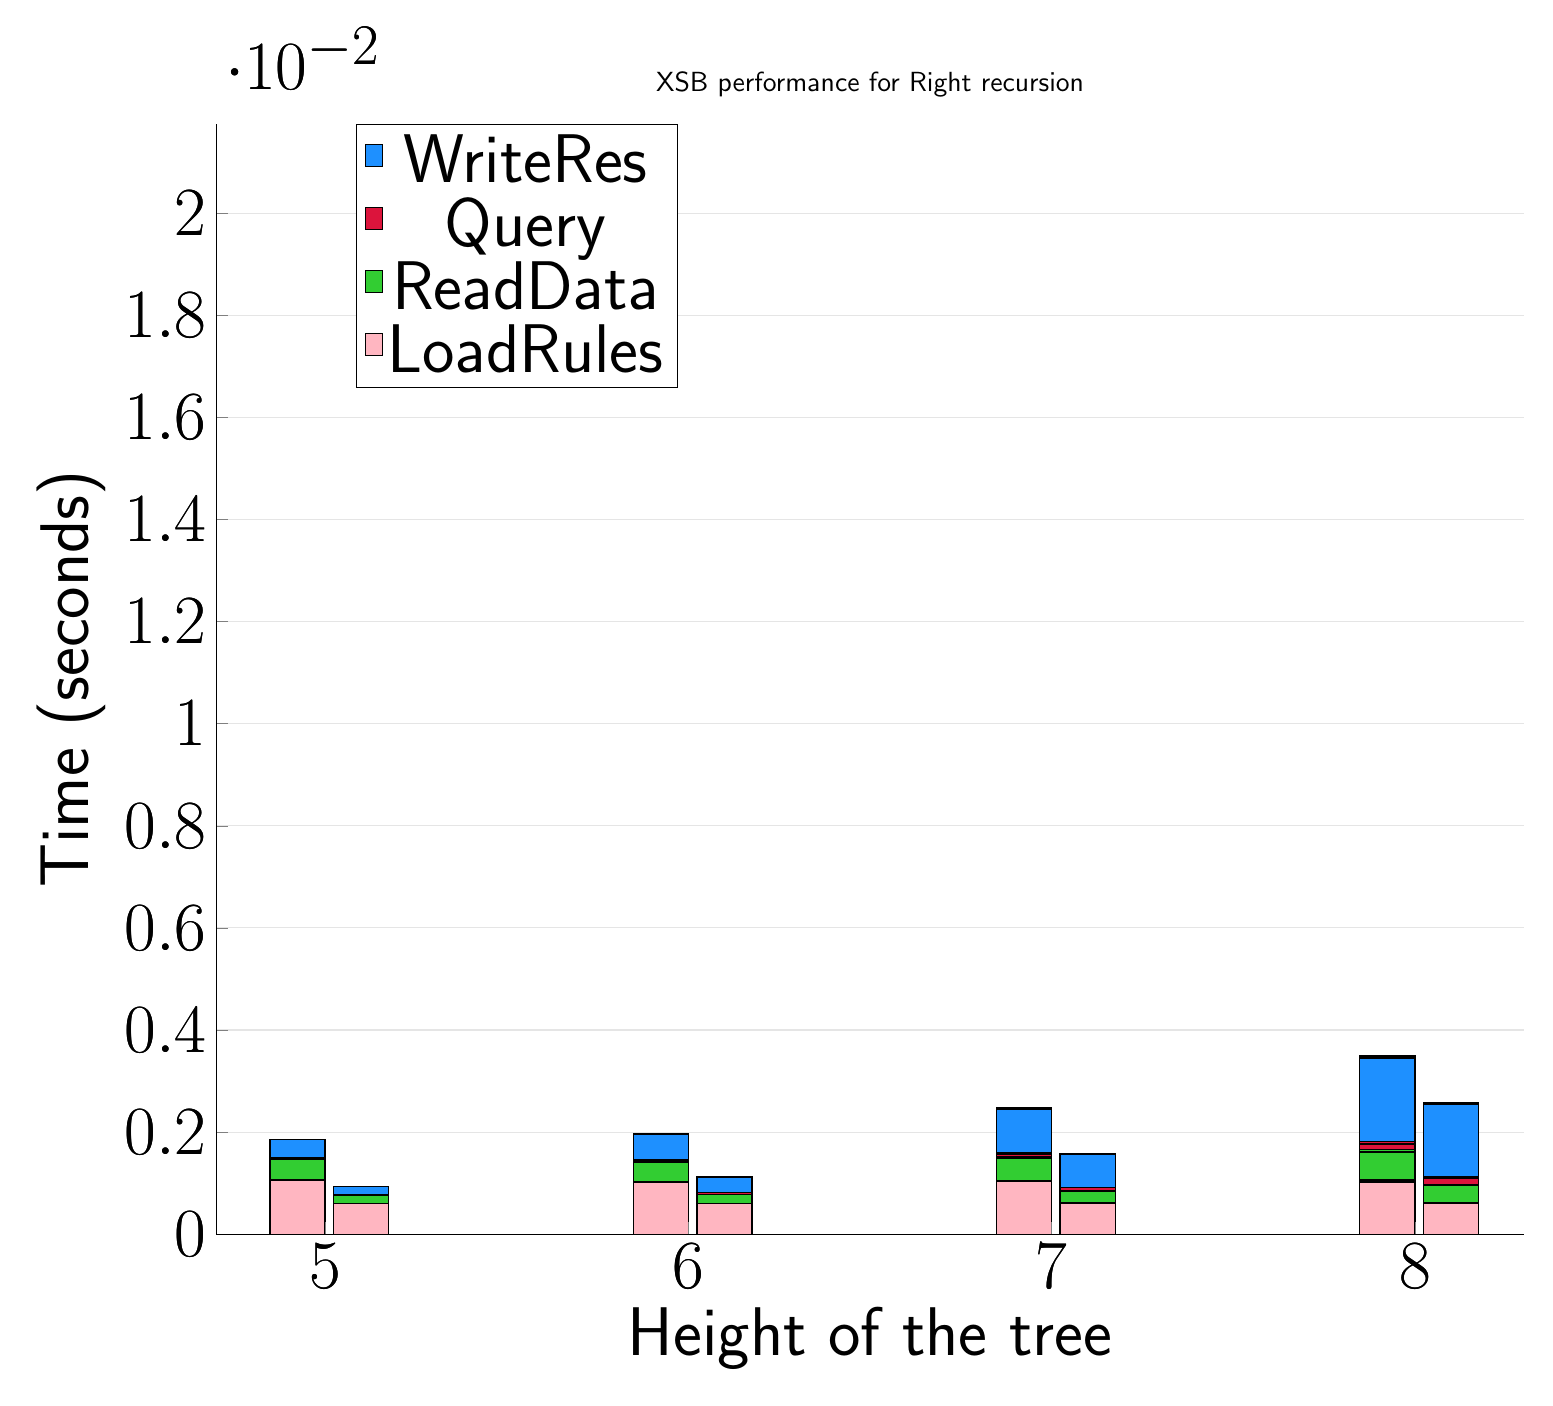
\begin{tikzpicture}
	\begin{axis}[
			ybar stacked,
			title={XSB performance for Right recursion},
			bar shift=-10pt,
			width=1.5\textwidth,
			bar width=0.7cm,
			ymajorgrids, tick align=inside,
			major grid style={draw=gray!20},
			xtick=data,
			ymin=0, ymax=0.02175771713256836,
			axis x line*=bottom,
			axis y line*=left,
			enlarge x limits=0.1,
			legend style={
					at={(0.23, 1)},
					anchor=north,
					legend columns=1,
					font=\Huge,
				},
			ylabel={Time (seconds)},
			xlabel={Height of the tree},
			label style={font=\Huge},
			tick label style={font=\Huge},
		]
		\addlegendimage{fill=DodgerBlue, draw=black, line width=0.2pt}
		\addlegendentry{WriteRes}
		\addlegendimage{fill=Crimson, draw=black, line width=0.2pt}
		\addlegendentry{Query}
		\addlegendimage{fill=LimeGreen, draw=black, line width=0.2pt}
		\addlegendentry{ReadData}
		\addlegendimage{fill=LightPink, draw=black, line width=0.2pt}
		\addlegendentry{LoadRules}
		\addplot +[fill=LightPink, draw=black, line width=0.5pt] coordinates {
				(5, 0.001059699058532715)
				(6, 0.0010242223739624031)
				(7, 0.001050591468811034)
				(7, 0.0010529756546020512)
				(7, 0.001038718223571778)
				(8, 0.001024889945983886)
				(8, 0.0010428667068481429)
				(8, 0.001071667671203614)
			};
		\addplot +[fill=LimeGreen, draw=black, line width=0.5pt] coordinates {
				(5, 0.0004057168960571289)
				(6, 0.0003907918930053712)
				(7, 0.0004380226135253907)
				(7, 0.00046164989471435546)
				(7, 0.00046696662902832013)
				(8, 0.000580000877380371)
				(8, 0.000568509101867676)
				(8, 0.0005859613418579102)
			};
		\addplot +[fill=Crimson, draw=black, line width=0.5pt] coordinates {
				(5, 2.636909484863281e-05)
				(6, 4.053115844726562e-05)
				(7, 7.479190826416014e-05)
				(7, 7.43865966796875e-05)
				(7, 7.398128509521483e-05)
				(8, 0.00015730857849121093)
				(8, 0.0001613140106201171)
				(8, 0.0001631736755371094)
			};
		\addplot +[fill=DodgerBlue, draw=black, line width=0.5pt] coordinates {
				(5, 0.0003592252731323243)
				(6, 0.0005072116851806641)
				(7, 0.0009206771850585943)
				(7, 0.0008712291717529299)
				(7, 0.0008685827255249023)
				(8, 0.0016872882843017572)
				(8, 0.0016997575759887707)
				(8, 0.0016780853271484385)
			};
	\end{axis}
	\begin{axis}[
			ybar stacked,
			bar shift=13pt,
			width=1.5\textwidth,
			bar width=0.7cm,
			ymajorgrids, tick align=inside,
			major grid style={draw=none},
			xtick=data,
			ymin=0, ymax=0.02175771713256836,
			axis x line*=none,
			axis y line*=none,
			enlarge x limits=0.1,
			label style={font=\Huge},
			tick label style={font=\Huge},
		]
		\addplot +[fill=LightPink, draw=black, line width=0.5pt] coordinates {
				(5, 0.0006007000000000003)
				(6, 0.0005972000000000003)
				(7, 0.0006123000000000003)
				(7, 0.0006026000000000006)
				(7, 0.0006090000000000004)
				(8, 0.0005976000000000003)
				(8, 0.0006092999999999999)
				(8, 0.0006185000000000001)
			};
		\addplot +[fill=LimeGreen, draw=black, line width=0.5pt] coordinates {
				(5, 0.00016139999999999978)
				(6, 0.00018269999999999978)
				(7, 0.00023829999999999972)
				(7, 0.0002412999999999998)
				(7, 0.00024109999999999982)
				(8, 0.0003510000000000001)
				(8, 0.0003514000000000001)
				(8, 0.00035729999999999974)
			};
		\addplot +[fill=Crimson, draw=black, line width=0.5pt] coordinates {
				(5, 2.2000000000000155e-05)
				(6, 3.6000000000000096e-05)
				(7, 6.960000000000042e-05)
				(7, 6.920000000000019e-05)
				(7, 6.950000000000014e-05)
				(8, 0.00014489999999999992)
				(8, 0.0001466)
				(8, 0.0001489000000000004)
			};
		\addplot +[fill=DodgerBlue, draw=black, line width=0.5pt] coordinates {
				(5, 0.0001561000000000001)
				(6, 0.00030479999999999944)
				(7, 0.0006472999999999997)
				(7, 0.0006433999999999997)
				(7, 0.0006484)
				(8, 0.001446)
				(8, 0.001462)
				(8, 0.0014440999999999996)
			};
	\end{axis}
\end{tikzpicture}

\end{document}
